\documentclass[10pt,twocolumn,letterpaper]{article}
\usepackage[margin=0.75in,columnsep=0.25in]{geometry}
\usepackage{times}
\usepackage[T1]{fontenc}
\usepackage{microtype}
\usepackage{amsmath,amssymb}
\usepackage{graphicx}
\usepackage{booktabs}
\usepackage[numbers,sort&compress]{natbib}
\usepackage{xcolor}
\usepackage[colorlinks=true,linkcolor=blue!60!black,citecolor=blue!60!black,urlcolor=blue!60!black]{hyperref}
\usepackage{caption}
\usepackage{enumitem}
\captionsetup{font=small,labelfont=bf}
\setlist{nosep,leftmargin=*}
\newcommand{\pvs}{\mathrm{PVS}}

\title{\Large\bfseries Entropy-Continuum Mechanics for Video:\\ Permanence Scoring and Frame-Shared Generation\\ \large Preliminary Results and Failure Modes}
\author{Krishna Sumanth Garlapati\\ \small Independent Researcher}
\date{\small Technical report, November 2026}

\begin{document}
\twocolumn[
\maketitle
\vspace{-1.2em}
\begin{center}
\begin{minipage}{0.86\textwidth}
\small
\textbf{Abstract.}
We model information in a video as a material that moves with the scene. Its local density is coding cost in bits. A balance law states that information is carried along the motion and created or destroyed only by a source term, which physically belongs at occlusion boundaries, frame edges and genuine new events. We study two uses of this view.
(i) The \emph{Permanence Violation Score} (PVS) measures information created or destroyed in open view. On synthetic clips with injected vanishing, melting, identity swaps and texture boiling, PVS separates violations from legal motion, occlusion and exit/entry with 0.86 ROC AUC, versus 0.63 for the standard warping error. Under JPEG compression and lighting changes it reaches 0.80, versus 0.51. Three choices proved necessary: measuring created \emph{content} rather than change of the scalar amount, locating occlusion boundaries from neighbouring frame pairs, and low-pass filtering against codec artifacts. On 15 clips from 8 video generators, however, PVS did not separate generated from real footage. Its strongest responses were to lighting effects, shot transitions and fast non-rigid motion.
(ii) In a small video diffusion transformer, we compute static-background tokens once and share them across frames. Each shared key receives a log-multiplicity attention bias (proportional attention), and the static map comes from a 2-step draft pass. This reproduces same-noise full compute at 41.5--43.8\,dB PSNR with 2.4--3.6$\times$ fewer FLOPs, which projects to 3.7--5.7$\times$ at the scale of current video transformers. Without the bias the same sharing reaches only $\sim$20\,dB. Token caching, freezing of settled tokens, and switching to sharing mid-generation all lost to simply using fewer sampling steps.
All experiments are toy-scale and CPU-only. We report them as evidence about mechanisms and as a record of what did not work.
\end{minipage}
\end{center}
\vspace{1.2em}
]

\section{Introduction}
Video generators fail in characteristic ways: objects melt into the background, vanish while in plain view, swap identity, or show textures that ``boil'' from frame to frame~\cite{huang2024vbench}. These are failures of \emph{permanence}. They are hard to measure with standard temporal-consistency metrics. Warping error~\cite{lai2018blind} masks out pixels that fail a forward--backward flow check~\cite{sundaram2010dense} as occluded, and those are often exactly the pixels where a violation happens. Generators also spend the same compute on every token, whether it shows a static wall or a moving hand.

We start from an analogy with continuum mechanics. A material is a distribution of mass that moves and obeys a conservation law. We ask whether information in video can be treated the same way. Taken literally, the analogy fails, and we document how. Made precise, it yields a balance law with a source term. That law gives one tool for measurement and one mechanism for compute reuse.

\paragraph{Contributions.}
\begin{itemize}
\item A balance-law view of video information (\S\ref{sec:framework}) and a training-free score, PVS, built on it (\S\ref{sec:pvs}).
\item Three design choices, each found by a failing test, without which the score does not work (\S\ref{sec:pvs-ablate}).
\item Frame-shared generation with proportional attention, together with an exactness argument. On a small model it reproduces full compute at 41--44\,dB with 2.4--3.6$\times$ fewer FLOPs, without an oracle (\S\ref{sec:compute}).
\item A record of negative results (\S\ref{sec:negative}): failure on real AI clips, scalar entropy, token caching and freezing versus fewer steps, mid-generation switching, and early abort.
\end{itemize}

\section{Related work}
\paragraph{Temporal consistency and video quality.} Warping error~\cite{lai2018blind} and the subject and background consistency dimensions of VBench~\cite{huang2024vbench} are the usual consistency metrics. FVD~\cite{unterthiner2018fvd} measures distribution-level quality. We compare against warping error because it is the closest per-clip, training-free alternative.
\paragraph{Flow and occlusion.} We use dense flow~\cite{farneback2003two}, with RAFT~\cite{teed2020raft} as a drop-in upgrade. Occlusion reasoning builds on forward--backward checks~\cite{sundaram2010dense} and on classic smoothness priors~\cite{horn1981determining}.
\paragraph{Information density.} Our density estimator is the LOCO-I/JPEG-LS predictor~\cite{weinberger2000loco}. Byte Latent Transformer~\cite{pagnoni2024blt} allocates compute by next-byte entropy, an instance of the ``compute $\propto$ information'' principle in text.
\paragraph{Diffusion and thermodynamics.} Diffusion models were derived from non-equilibrium thermodynamics~\cite{sohl2015deep}. We use rectified flow~\cite{liu2023flow,lipman2023flow}. Per-token noise levels appear in Diffusion Forcing~\cite{chen2024diffusion}. Correlated noise across frames has been used as a video prior~\cite{ge2023preserve}.
\paragraph{Token merging.} ToMe~\cite{bolya2023token,bolya2023tomesd} merges similar tokens and introduced proportional attention, the log-size bias we reuse. VidToMe~\cite{li2024vidtome} merges tokens across frames for video editing. Our sharing differs in three ways. It is decided before generation from a draft pass. It removes tokens from the sequence rather than averaging them. And we test it against exact full compute from the same noise. The individual ingredients are not new; our contribution is their combination and the measurement.

\section{Framework}\label{sec:framework}
Let $I_t$ be frame $t$ and $v_t$ the flow from $t$ to $t{+}1$. We define the local information density as coding cost,
\begin{equation}
\iota(x,t) = -\log_2 p\big(I_t(x)\mid \text{causal neighbourhood}\big),
\end{equation}
and posit a balance law with a source term $s$:
\begin{equation}
\partial_t \iota + \nabla\!\cdot(\iota\, v) = s .
\end{equation}
Unlike mass, information is not conserved. Real video creates it at disocclusions, objects entering the frame, and genuine events such as splashes or flames. Physics restricts \emph{where} $s\neq 0$ may occur: along motion boundaries, where one surface passes another, and at frame edges. A permanence violation is a source or sink anywhere else.
\paragraph{Temperature.} In diffusion sampling the noise level plays the role of temperature~\cite{sohl2015deep}. Regions can ``cool'' (settle) at different rates, and guidance acts as cooling. We use this view to motivate per-region freezing (\S\ref{sec:compute}), and later test whether it holds up.

\section{Permanence Violation Score}\label{sec:pvs}
\paragraph{Density.} $\iota$ is the bits per pixel of the MED predictor residual~\cite{weinberger2000loco}, coded with a discretised Laplacian whose scale is the local mean absolute residual.
\paragraph{Source term (content form).} We use the Lagrangian form and measure \emph{created content}: the excess bits needed to explain frame $t{+}1$ given motion-compensated frame $t$. Let $r(x)=I_{t+1}(x+v(x))-I_t(x)$ and let $b=\mathrm{median}|r|/\ln 2$ be the robust Laplacian noise scale. Then
\begin{equation}
s(x,t)=\max\!\Big(\tfrac{|r(x)|}{b\ln 2}-\log_2 e,\;0\Big),
\end{equation}
i.e.\ the Laplacian code length of $r$ minus the entropy of the noise itself, $\log_2(2eb)$,
so motion explained by noise alone costs nothing.
\paragraph{Where sources are legal.} The legal set $\mathcal{A}_t$ is the union of the frame-edge band and the motion-boundary bands. Motion boundaries are pixels with $\|\nabla v\|>\tau$, dilated by the local 99th-percentile speed plus 3\,px. Crucially, they are computed from the \emph{neighbouring} pairs $(t{-}1,t)$ and $(t{+}1,t{+}2)$, not from the pair being judged (\S\ref{sec:pvs-ablate}).
\paragraph{Score.} With dead zone $\delta$,
\begin{equation}
\pvs_t=\frac{\sum_{x\notin\mathcal{A}_t}\max(|s(x,t)|-\delta,0)}{\sum_x \iota(x,t)},
\end{equation}
and the clip score is $\pvs=\max_t \pvs_t$.
The map inside the sum localises the violation (Fig.~\ref{fig:sanity}). For compressed footage, frames are first blurred with a Gaussian of $\sigma{=}2$\,px. We also tested a \emph{vector} variant: the per-pixel change of a 9-channel entropy fingerprint (tone plus 8 oriented band energies, gain-normalised) along the flow. A \emph{combined} variant takes the geometric mean of the content and vector sources.

\begin{figure*}[t]
\centering
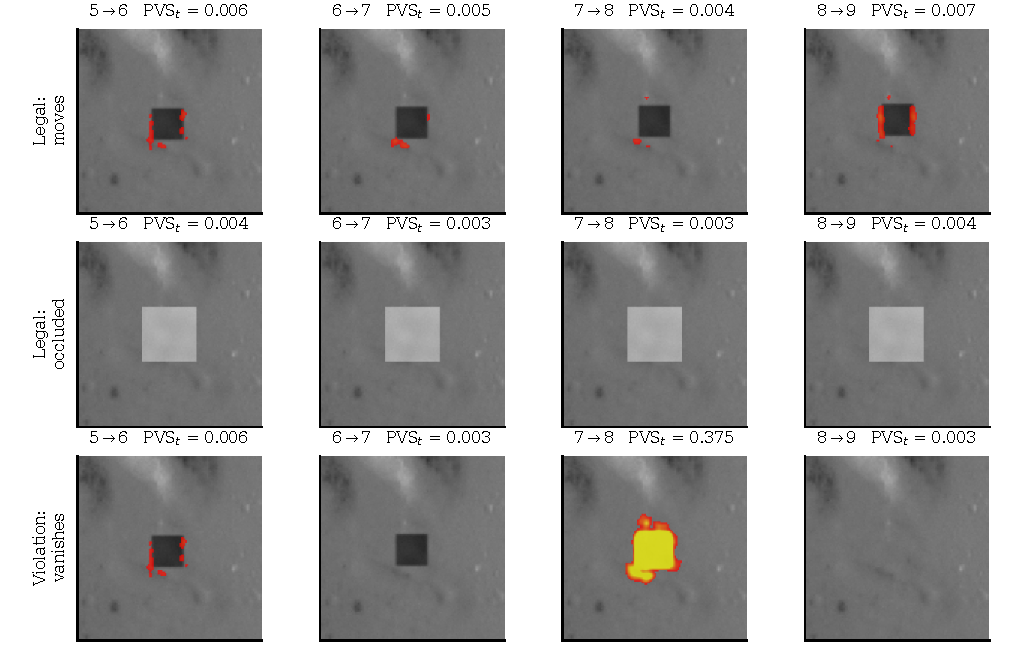
\includegraphics[width=\textwidth]{figs/fig_sanity.pdf}
\caption{PVS heatmaps (red/yellow: bits created or destroyed outside legal zones, shown where $>$0.5) on synthetic sanity clips that share one background. Legal motion and occlusion stay quiet ($\pvs_t\approx$0.003--0.007). The vanish is caught at the exact transition, at 0.375.}
\label{fig:sanity}
\end{figure*}

\subsection{Synthetic benchmark}
\paragraph{Data.} Clips have 16 frames at 128$\times$128. The backgrounds are natural textures from the scikit-image sample set; half the clips have a camera pan. One textured sprite moves with sub-pixel motion. \emph{Legal} events: plain motion, passing behind an occluder, fully exiting or entering the frame, and (in A1b) a global brightness drift with a moving soft shadow. \emph{Violations}: vanish or appear in open view (abrupt or a 4-frame fade), melt (progressive blur and fade), identity swap, and texture boiling. Thresholds were tuned on 5 sanity seeds and the prefilter on a separate dev set; all reported numbers are on disjoint held-out seeds.

\begin{table}[t]
\centering\small
\caption{ROC AUC, violation vs.\ legal (A1: 360 clips; A1b: 300 clips, half JPEG $q{=}35$, with legal lighting changes, prefilter $\sigma{=}2$).}
\label{tab:detect}
\begin{tabular}{@{}lccc@{}}
\toprule
 & A1 all & A1b all & A1b JPEG \\
\midrule
Warping error~\cite{lai2018blind} & 0.63 & 0.51 & 0.53 \\
Scalar density balance & 0.57 & 0.66 & 0.63 \\
PVS vector fingerprint & -- & 0.75 & 0.74 \\
PVS combined & -- & 0.80 & 0.77 \\
\textbf{PVS content (ours)} & \textbf{0.86} & \textbf{0.80} & \textbf{0.77} \\
\bottomrule
\end{tabular}
\end{table}

\begin{figure*}[t]
\centering
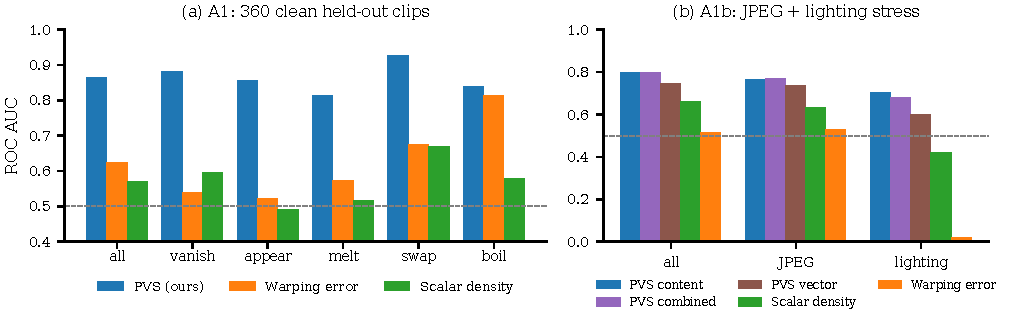
\includegraphics[width=\textwidth]{figs/fig_detection.pdf}
\caption{Detection AUC by violation type (a) and under stress (b). Against legal lighting changes, warping error inverts (0.02 AUC): it scores the lighting clips as \emph{worse} than the true violations.}
\label{fig:detect}
\end{figure*}

\paragraph{Results.} Table~\ref{tab:detect} and Fig.~\ref{fig:detect} summarise the results. On A1, PVS reaches 0.94 AUC with a static camera and 0.79 with a pan. 72\% of the flagged mass falls inside the dilated event region, which covers 5.1\% of the frame, and the worst frame is the event frame in 95\% of violations (boiling excluded, since its window covers most of the clip). The main weakness is false alarms: at 80\% recall, 22--28\% of legal clips are flagged.

\subsection{What was necessary}\label{sec:pvs-ablate}
\begin{enumerate}
\item \textbf{Content, not amount.} The direct analogue of mass conservation tracks the scalar $\iota$ along the flow. It fails (0.57 AUC), because a vanished object is replaced by background of similar density. In one case it went from 3.6 to 4.2 bits/px.
\item \textbf{Boundaries from neighbouring pairs.} Flow estimated across a violation invents motion to explain it. The resulting spurious motion boundaries mark the violation itself as a legal occlusion. With boundaries from the judged pair, the vanish sanity test was detected in 0/5 seeds; with neighbouring pairs, in 5/5.
\item \textbf{Prefiltering.} JPEG block artifacts look like created content. On a dev set, a $\sigma{=}2$ blur raised AUC on compressed clips from 0.61 to 0.78.
\end{enumerate}
Vector entropy beats scalar entropy but not the content form (Table~\ref{tab:detect}). Without prefiltering it helped on uncompressed clips (0.76 vs.\ 0.77 content, 0.81 combined), but the advantage disappeared once the prefilter was used.

\subsection{Real footage and real generators}
We scored four real or CGI clips (the scikit-video samples) and 15 generated clips. The generated clips cover two prompts, night-time dance crews and a skateboarder, from Runway Alpha, HunyuanVideo, Pika 2.2, Luma Ray 2, Sora, Veo 2, Veo 3 and Wan 2.1, taken from a public human-preference dataset. Peak PVS for the AI clips ranged from 0.19 to 2.22 (median 0.46); for the real clips it ranged from 0.64 to 1.25. \textbf{There was no separation.} The highest AI scores came from lighting effects (Veo 3), a cross-dissolve between shots (Veo 2), and fast non-rigid motion (dancing, skateboarding; Fig.~\ref{fig:realai}). On real footage, PVS also responded to changing facial expressions and a deforming cartoon body, and compression doubled the peak for identical content. The synthetic benchmark contained only rigid sprites and no edits, so it did not anticipate any of these.

\begin{figure*}[t]
\centering
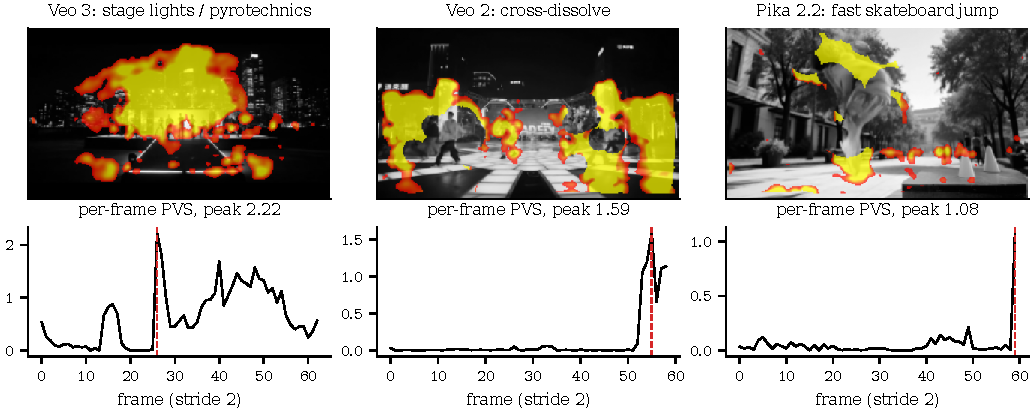
\includegraphics[width=\textwidth]{figs/fig_real_ai.pdf}
\caption{Highest PVS responses on generated clips. Lighting effects, a shot transition and fast non-rigid motion dominate. These are failure modes of the score, not confirmed violations by the generator.}
\label{fig:realai}
\end{figure*}

\section{Compute reuse}\label{sec:compute}
\paragraph{Model and protocol.} We use a video diffusion transformer with 1.1M parameters (4 layers, width 128, adaLN time conditioning), trained with rectified flow~\cite{liu2023flow} for 12k steps on a CPU. Clips have 8 frames at 32$\times$32 with 8$\times$8 patches, giving 128 tokens with full spatio-temporal attention. The training data are synthetic static-camera clips: smooth backgrounds with 1--2 textured moving sprites. Sampling is 20 Euler steps. Fidelity is the PSNR of a method's output against full compute from the same starting noise. For calibration, 10 steps instead of 20 gives 34.3\,dB, and 40 steps gives 39.2\,dB. Cost is counted with an analytic FLOP model of every forward call. We also \emph{project} each method's token fractions to a 75.6k-token, 40-layer, width-3072 video DiT, where attention dominates; this is a FLOP calculation, not a measurement. The sample quality of this model is limited (patch seams are visible), so the tests measure fidelity to full compute, not realism.

\paragraph{Methods.}
\emph{Token caching}: after a 25\% warm-up, only the top-$p$ tokens by density and motion are recomputed; the rest reuse cached keys, values and velocity.
\emph{Freezing}: a token stops being recomputed once the change of its predicted clean value between consecutive steps falls below $\tau$ (``delta'' rule), or that change times the current temperature $1{-}t$ does (``heat'' rule).
\emph{Frame sharing}: static positions are computed in one leader frame and removed from the sequence elsewhere; their outputs are copied.

\paragraph{Proportional attention makes sharing exact.} Suppose $m_j$ identical copies of key/value $(k_j,v_j)$ are collapsed into one. For any query $q$,
\begin{equation}
\frac{\sum_j m_j e^{q\cdot k_j}v_j}{\sum_j m_j e^{q\cdot k_j}}=\mathrm{softmax}_j\big(q\cdot k_j+\log m_j\big)\,v_j ,
\end{equation}
so adding $\log m_j$ to the logits reproduces full attention \emph{exactly} whenever the copies are identical~\cite{bolya2023token}. Copies are identical when the static positions start from the same noise and remain static. We therefore (1) run a 2-step draft, (2) mark positions whose maximum frame-to-frame change in the draft is below a threshold, and (3) generate from scratch with those positions sharing noise and compute from step 0. The draft's cost is included in all reported speedups.

\begin{table}[t]
\centering\small
\caption{Speed vs.\ fidelity on the tiny model. Speedup is measured in FLOPs; ``proj.'' projects the same token fractions to a 75.6k-token video DiT. $^\dagger$Compared with full compute from the same shared starting noise.}
\label{tab:speed}
\setlength{\tabcolsep}{2.5pt}
\resizebox{\columnwidth}{!}{%
\begin{tabular}{@{}lccc@{}}
\toprule
Method & Speedup & Proj. & PSNR (dB) \\
\midrule
Fewer steps (20$\to$7 / 20$\to$5) & 2.9 / 4.0 & same & 30.0 / 27.0 \\
Token caching, density+motion & 2.3 / 3.1 & same & 30.4 / 28.8 \\
Freezing, heat rule & 2.9 / 4.1 & same & 25.5 / 24.2 \\
10 steps + heat freezing & 3.1 / 4.0 & same & 30.5 / 28.5 \\
Sharing (8 fr.), plain attention$^\dagger$ & 2.7 & 5.3 & 20.2 \\
Sharing (8 fr.) + prop.\ attn., oracle$^\dagger$ & 2.7 & 5.3 & 43.6 \\
\textbf{Sharing + prop.\ attn., 2-step draft}$^\dagger$ & \textbf{2.4 / 3.6} & \textbf{3.7 / 5.7} & \textbf{43.8 / 41.5} \\
Sharing switched on mid-generation & 1.2--1.4 & 1.4--1.6 & 24--30 \\
\bottomrule
\end{tabular}}
\end{table}

\begin{figure}[t]
\centering
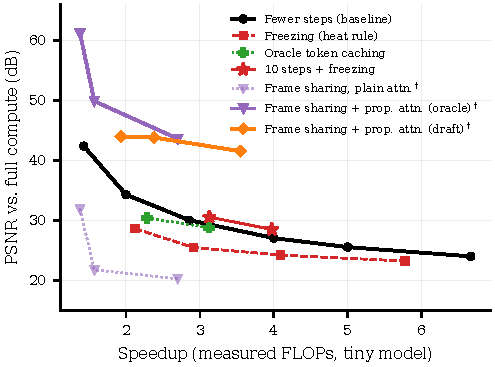
\includegraphics[width=\columnwidth]{figs/fig_speed.pdf}
\caption{Speed vs.\ fidelity. Only frame sharing with proportional attention lies clearly above the fewer-steps baseline. Stacking freezing on top of fewer steps gains $\sim$1.5\,dB.}
\label{fig:speed}
\end{figure}

\paragraph{Results.} Table~\ref{tab:speed} and Fig.~\ref{fig:speed} show the comparison. Draft-pass sharing shares 73--90\% of positions and stays within 37\,dB of same-noise full compute on every clip (worst case). Proportional attention is the difference between 20\,dB and 44\,dB at the same speedup. The settling measurement supports the temperature view qualitatively: the median settling step is 4 of 20 for static tokens and 7 for moving ones, and settling time correlates with density (Spearman 0.70). Exploiting it through freezing, however, lost to fewer steps at every speedup. Only stacking freezing on 10 steps beat the baseline, by 1.2--1.5\,dB.

\paragraph{The open question.} Shared noise yields a \emph{different} sample than independent noise; PSNR against the original output is 11--15\,dB. Whether the shared-noise sample is as good is untested. Its PVS rose from 0.70 to 1.1--1.3, but PVS is unreliable at 32\,px (\S\ref{sec:negative}). One plausible failure is an object that cannot move into a region marked static.

\section{Negative results}\label{sec:negative}
\begin{itemize}
\item \textbf{Real AI vs.\ real footage}: no separation (\S4.3).
\item \textbf{Scalar entropy as mass}: 0.57 AUC (\S\ref{sec:pvs-ablate}).
\item \textbf{Token caching and freezing} each lost to simply taking fewer steps (Table~\ref{tab:speed}).
\item \textbf{Mid-generation sharing}: the static map read from an early prediction marks too many positions as static, and switching resets each copy's trajectory. With 24--48\% of positions shared it reached 24--30\,dB, below the baseline.
\item \textbf{Cutting weak attention links}: static queries attend to moving keys at 0.73$\times$ the uniform rate (0.41$\times$ in the last layer). Masking those links costs quality (27.9\,dB).
\item \textbf{Early abort}: PVS of the step-2 to step-6 prediction does not predict the final PVS (Spearman $\approx$0).
\item \textbf{PVS at 32\,px}: generated and training clips are not separated (AUC 0.53). Small moving textures change appearance between sub-pixel positions (aliasing), which sets a false-alarm floor.
\end{itemize}

\section{Limitations}
Every result is toy-scale. The detection benchmark is synthetic with rigid sprites; the generator has 1.1M parameters and visible artifacts; and the real-clip test is 19 clips without human labels. The projected speedups are FLOP calculations that ignore memory traffic and kernel overheads. Frame sharing assumes a static camera, and its sample quality under shared noise is unknown. Hyperparameters were tuned on small dev sets. We have not compared against the VBench consistency scores or against learned detectors.

\section{Conclusion and next steps}
The materials analogy is productive once it is made precise. Information is not conserved, but \emph{where} it may be created is constrained. That constraint yields a working permanence score on controlled data and an exact compute-reuse mechanism. On real generated video the score is not yet useful. The next steps are, in order:
\begin{enumerate}
\item Test whether shared-noise samples lose quality on an open video model (blind preference, FVD).
\item Port draft-pass sharing with proportional attention to that model and measure wall-clock time.
\item For PVS: add shot-cut detection, model lighting changes, handle non-rigid motion with stronger flow, and validate against human melting ratings.
\end{enumerate}

\paragraph{Reproducibility.} Code, data generators, results (JSON) and the figure script for every number in this report are in the accompanying repository (\texttt{ecm-video}). Each table entry names its source script in \texttt{FINDINGS.md}.

\paragraph{Acknowledgements.} Experiments, code and drafting were carried out with the help of an AI assistant (Claude, Anthropic). An independent automated code review found four bugs, which were fixed before the reported numbers were produced.

\small
\begin{thebibliography}{99}
\bibitem{bolya2023token} D.~Bolya, C.-Y. Fu, X.~Dai, P.~Zhang, C.~Feichtenhofer, and J.~Hoffman. Token merging: Your ViT but faster. In \emph{ICLR}, 2023.
\bibitem{bolya2023tomesd} D.~Bolya and J.~Hoffman. Token merging for fast stable diffusion. In \emph{CVPR Workshops}, 2023.
\bibitem{chen2024diffusion} B.~Chen, D.~Mart\'i Mons\'o, Y.~Du, M.~Simchowitz, R.~Tedrake, and V.~Sitzmann. Diffusion forcing: Next-token prediction meets full-sequence diffusion. In \emph{NeurIPS}, 2024.
\bibitem{farneback2003two} G.~Farneb\"ack. Two-frame motion estimation based on polynomial expansion. In \emph{SCIA}, 2003.
\bibitem{ge2023preserve} S.~Ge et al. Preserve your own correlation: A noise prior for video diffusion models. In \emph{ICCV}, 2023.
\bibitem{horn1981determining} B.~K.~P. Horn and B.~G. Schunck. Determining optical flow. \emph{Artificial Intelligence}, 17:185--203, 1981.
\bibitem{huang2024vbench} Z.~Huang et al. VBench: Comprehensive benchmark suite for video generative models. In \emph{CVPR}, 2024.
\bibitem{lai2018blind} W.-S. Lai, J.-B. Huang, O.~Wang, E.~Shechtman, E.~Yumer, and M.-H. Yang. Learning blind video temporal consistency. In \emph{ECCV}, 2018.
\bibitem{li2024vidtome} X.~Li, C.~Ma, X.~Yang, and M.-H. Yang. VidToMe: Video token merging for zero-shot video editing. In \emph{CVPR}, 2024.
\bibitem{lipman2023flow} Y.~Lipman, R.~T.~Q. Chen, H.~Ben-Hamu, M.~Nickel, and M.~Le. Flow matching for generative modeling. In \emph{ICLR}, 2023.
\bibitem{liu2023flow} X.~Liu, C.~Gong, and Q.~Liu. Flow straight and fast: Learning to generate and transfer data with rectified flow. In \emph{ICLR}, 2023.
\bibitem{pagnoni2024blt} A.~Pagnoni et al. Byte latent transformer: Patches scale better than tokens. \emph{arXiv:2412.09871}, 2024.
\bibitem{sohl2015deep} J.~Sohl-Dickstein, E.~Weiss, N.~Maheswaranathan, and S.~Ganguli. Deep unsupervised learning using nonequilibrium thermodynamics. In \emph{ICML}, 2015.
\bibitem{sundaram2010dense} N.~Sundaram, T.~Brox, and K.~Keutzer. Dense point trajectories by GPU-accelerated large displacement optical flow. In \emph{ECCV}, 2010.
\bibitem{teed2020raft} Z.~Teed and J.~Deng. RAFT: Recurrent all-pairs field transforms for optical flow. In \emph{ECCV}, 2020.
\bibitem{unterthiner2018fvd} T.~Unterthiner, S.~van~Steenkiste, K.~Kurach, R.~Marinier, M.~Michalski, and S.~Gelly. Towards accurate generative models of video: A new metric \& challenges. \emph{arXiv:1812.01717}, 2018.
\bibitem{weinberger2000loco} M.~J. Weinberger, G.~Seroussi, and G.~Sapiro. The LOCO-I lossless image compression algorithm: Principles and standardization into JPEG-LS. \emph{IEEE Trans.\ Image Processing}, 9(8):1309--1324, 2000.
\end{thebibliography}
\end{document}
